\begin{figure}
    \centering
    \begin{subfigure}{0.3\textwidth}
        \centering
        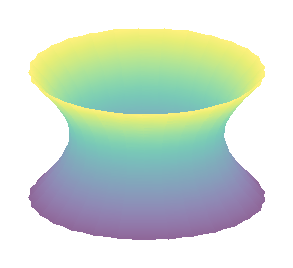
\begin{tikzpicture}[scale=0.6]
            \begin{axis}[
                    view={30}{30},
                    axis lines=none,
                    colormap/viridis,
                    samples=30,
                    domain=-1:1,
                    y domain=-2*pi:2*pi
            ]
            \addplot3[
                surf,
                shader=interp,
                opacity=.6,
                    z buffer=sort
            ] ({0.2+cosh(x)*cos(deg(y))},
            {0.2+cosh(x)*sin(deg(y))},
            {sinh(x)});     
            \end{axis}
        \end{tikzpicture}
        \caption{Negative curvature}
     \end{subfigure}
     \hfill
     \begin{subfigure}{0.3\textwidth}
        \centering
        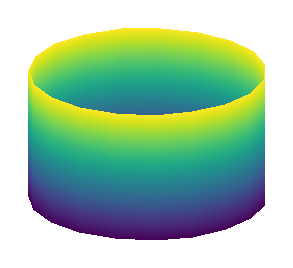
\begin{tikzpicture}[scale=0.6]
            \begin{axis}[
                    view={30}{30},
                    axis lines=none,
                    colormap/viridis,
                    samples=20,
                    domain=0:2*pi,
                    y domain=-2*pi:2*pi
            ]
            \addplot3[
                    surf,
                    shader=interp,
                    z buffer=sort
            ] ({cos(deg(x))},
            {sin(deg(x))},
            {y});
            \end{axis}
        \end{tikzpicture}
        \caption{Zero curvature.}
     \end{subfigure}
     \hfill
     \begin{subfigure}{0.3\textwidth}
        \centering
        
\begin{tikzpicture}[scale=0.6]
            \begin{axis}[
                    view={30}{0},
                    axis lines=none,
                    colormap/viridis,
                    samples=20,
                    domain=-90:90,
                    y domain=0:360
            ]
            \addplot3[
                    surf,
                    shader=interp,
                    z buffer=sort
            ]
            ({cos(x)*cos(y)},
            {cos(x)*sin(y)},
            {sin(x)});
            \end{axis}
        \end{tikzpicture}
        \caption{Positive curvature}     
    \end{subfigure}
    \caption{Surfaces with various curvatures.}
    \label{fig:spaceCurvatures}
\end{figure}